\documentclass[../phys-f308.tex]{subfiles}

\begin{document}
    \part{Intermolecular forces}
    \begin{abstract}
        In the study of matter, one defines several different states. In this course, we will focus on the study of the properties of condensed matter. Crystals and liquids are examples of such condensed matter - the interaction between molecules of the latter is of the order of $E_{int}>> k_BT$ whereas the former presents an interaction energy $E_{int}\geq k_BT$ which can be put in contrast to a gas' $E_{int}<< k_BT$. Let us note that thermal energy is much larger than the interactions between particules in the gaseous states. 
    \end{abstract}

    \section{Microscopic interaction potential}

    Let us consider the interaction between two different molecules. The total energy in the system can be written as
    \begin{equation}
        E_{tot}(r) = E_A+E_B+w(r)
    \end{equation}
    where $r$ is the distance between the molecules $A$ and $B$ and $w(r)$ is the \emph{potential of interaction}, defined as
    \begin{align}
        w(r) &= E_{tot}(r) - E_{tot}(\infty)\\
        w(r) &= -\int_r^{\infty}F(r)dr \quad \Leftrightarrow \quad F(r) = -\frac{dw}{dr}\label{eq: F dw/dr}
    \end{align}
    Beware to the minus sign between the two: the interaction is \emph{attractive} when the potential is negative, and \emph{repulsive} when the potential   

    \section{Molecular interactions via electrostatic potentials}

    We will perform a review of the electrostatic potential interaction, with an increasing level of complexity. In particular, we will consider the interaction between...
    \begin{itemize}
        \item Two single point charges (approximation for two ions), dipole moments (approximation for two molecules)
        \item A single point charge and a non-rotating dipole moment
        \item Two non rotating dipole moments
        \item A single point charge and a rotating dipole moment
        \item Two rotating dipole moments
    \end{itemize}

    \subsection{Electrostatic interaction between two point charges}
    Let us consider two single points charges $Q_1$ and $Q_2$ separated by a distance $r$. As a reminder, let us note that the electric field of a charge $Q$ at a distance $r$ is given by $E = \frac{Q}{4\pi\epsilon_r\epsilon_0 r^2}$. Therefore, the electric force of charge $Q_1$ on charge $Q_2$ is given by $F=E_1Q_2 = \frac{Q_1Q_2}{4\pi\epsilon_r\epsilon_0 r^2} = \frac{z_1z_2 e^2}{4\pi\epsilon_r\epsilon_0 r^2}$ by introducing the valence numbers $z_i$. We deduce the macroscopic electrostatic potential
    \begin{equation}
        w(r) = -\frac{z_1z_2e^2}{4\pi\epsilon_r\epsilon_0 r}
    \end{equation} 

    \subsubsection{Electrostatic interaction: application to $NaCl$}

    In a vaccum, one finds that $w_{NaCl} = -8.4\ti 10^{-19}J$. However, at room temperature one has that $U_T = k_BT \approx 1.38\ti 10^{-23} J/K \cdot 291 J = 4\ti 10^{-21}J$. Given that \color{red}$w_{NaCl}>200 k_BT$\footnote{Why do we ignore the negative sign?}\color{black}, NaCl is stable at room temperature in a vaccum. However, put it in a medium with high dielectric constant such as water and $w_{NaCl}^{H_2O}(r) \approx 2.5 k_BT$.

    \subsection{Dipole moments}

    Asymetric molecules bounded by covalent bounds often contains dipole moments. One defines the units of $Debye$ for this purpose: take two charges $e$ and $-e$ separated by a distance of one $Angstrum$:
    \begin{equation*}
        \mu = 4.8 D
    \end{equation*}

    \subsubsection{Dipole moment of water}

    \begin{example}
        The molecule of water can be seen as two $OH$ molecules separated by an angle of $104.5°$. Given that $\mu_{OH} = 1.51 D$, we deduce that the dipole moment of water is given by 
        \begin{equation}
            \mu_{H_2O} = 2\cos\left(\frac{H\hat{O}H}{2}\right)\mu_{HO} = 1.85D
        \end{equation}
    \end{example}

    \subsection{Ion-dipole interaction}\label{sec: ion-dipole interaction}

    Instead of looking a two single point charges and a dipole seperately, let us put them together and see what happens as shown in figure \ref{fig: ion-dipole interaction}. The resulting macroscopic electrostatic potential is
    \begin{equation}
        w(r) = -\frac{qQ}{4\pi\epsilon_0r_A}+\frac{qQ}{4\pi\epsilon_0r_B} = \frac{qQ}{4\pi\epsilon_0}\left(\frac{1}{r_B}-\frac{1}{r_A}\right)\label{eq: ion-dipole interaction 1}
    \end{equation}

    Let us note that $r_A \approx r-\frac{l}{2}\cos\theta$ whereas $r_B\approx r+\frac{l}{2}\cos\theta$. Applying the approximation $\frac{r_A-r_B}{r_Ar_B}\approx -\frac{l\cos\theta}{r^2}$, one finds that  \eqref{eq: ion-dipole interaction 1} can be rewritten as
    
    \begin{equation}
        w(r) \approx -\frac{qQ}{4\pi\epsilon_0}\frac{l\cos\theta}{r^2} = -\mu\frac{Q\cos\theta}{4\pi\epsilon_0r^2} \quad w(r) = -\mu E(r)\cos\theta
    \end{equation}

    The potential is either attractive or repulsive, depending on the orientation of the molecule.

    \begin{figure}[H]
        \centering
        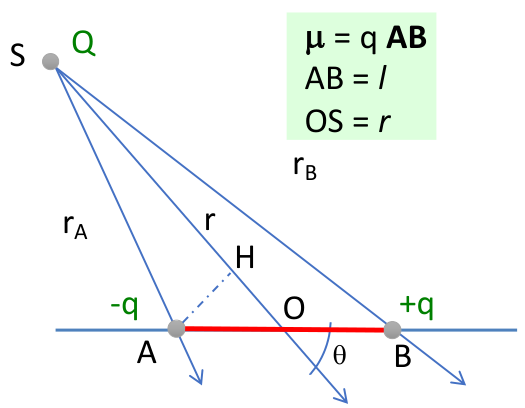
\includegraphics[width=50mm]{partA/Pictures/DipoleIon.png}
        \caption{Ion-dipole interaction}
        \label{fig: ion-dipole interaction}
    \end{figure}

    \subsection{Dipole-dipole interaction}\label{sec: DDipole interaction}

    Assuming the two dipoles can freely move in the $xyz$ space, one would need to replace the angle $\theta$ used previously by three different angles - $\theta_1,\theta_2$ and $\varphi$ as shown in figure \ref{fig: DDipole}. The interaction potential can then be written as
    \begin{equation}
        w(r,\theta_1,\theta_2,\varphi) = -\frac{\mu_1\mu_2}{4\pi\epsilon_o\epsilon_r r^3}\left(2\cos\theta_1\cos\theta_2-\sin\theta_1\sin\theta_2\cos\varphi\right)
    \end{equation}

    To simplify the problem, let us assume the angles $\theta_1$ is equal to $0$, meaning that the only allowed variation is in $\theta_2$ and in the rotation angle $\varphi$. Then,
    \begin{itemize}
        \item $\theta_2 = 0 \quad \Leftrightarrow \quad w(r,0,0,\varphi) = -\frac{2\mu_1\mu_2}{4\pi\epsilon_r\epsilon_0 r^3}$. The two dipoles are attracted to each other.
        \item $\theta_2 = 90$. The dipoles are neither attracted nor repulsed by each other - they are said to be neutral. 
        \item $\theta_2 = 180$. The dipoles are repelled by each other. 
        \item $\theta_2 = 270$. The dipoles are neither attracted nor repulsed by each other - they are said to be neutral.
    \end{itemize}
        Let us note that in all situations, if the dipoles are free to rotate, then they tend to align themselves (situation with the lowest potential). This is shown in figure \ref{dif: DDipole theta1 = 0}.
    
    \begin{figure}[H]
        \begin{subfigure}{.5\textwidth}
            \centering
            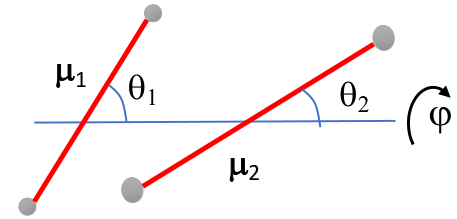
\includegraphics[width=50mm]{partA/Pictures/DDipole.png}
            \caption{Dipole-Dipole interaction}
            \label{fig: DDipole}
        \end{subfigure}
        \begin{subfigure}{.5\textwidth}
            \centering
            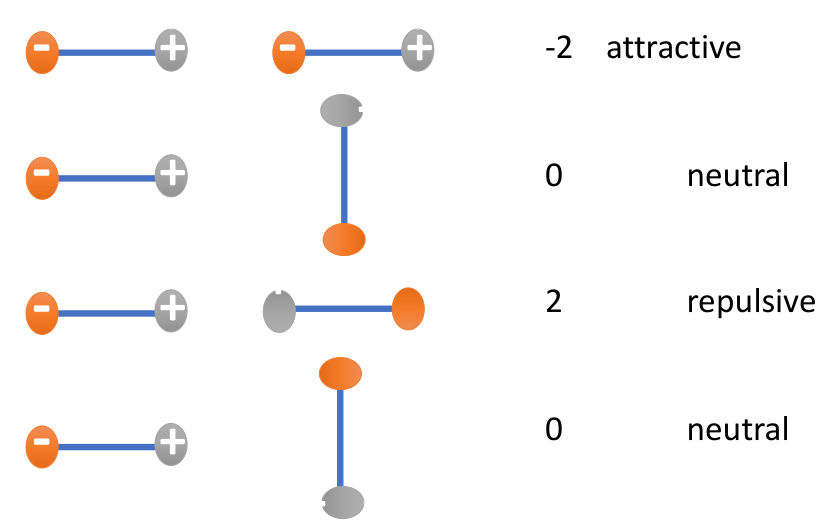
\includegraphics[width=50mm]{partA/Pictures/DDipole_interactions.png}
            \caption{Summary of the different possible states with $\theta_1 = 0$.}
            \label{dif: DDipole theta1 = 0}
        \end{subfigure}
    \end{figure}

    \subsection{Interactions involving freely rotating molecules}

    To take into account all different orientations, one would need to average the potential over the solid angle. Unfortunately, that is difficult to obtain analytically. How can we appropriately approximate the consequences of all the angles? Let us average all the possible orientations over the solid angle $\Omega$.

    \begin{equation}
        e^{-\frac{w(r)}{kT}} = \frac{\int e^{-\frac{w(r,\Omega)}{kT}}d\Omega}{\int d\Omega} = \Bigg\langle e^{-\frac{w(r,\Omega)}{kT}}\Bigg\rangle
    \end{equation}

    When $kT>>w(r,\Omega)$, one finds
    \begin{equation}
        \Bigg\langle\exp\left[-\frac{w(r,\Omega)}{kT}\right]\Bigg\rangle = \Bigg\langle 1 - \frac{w(r,\Omega)}{kT} + \frac{1}{2}\left[\frac{w(r,\Omega)}{kT}\right]^2 + (...)\Bigg\rangle
    \end{equation}

    As the potential is expanded over a Taylor series, it looses its angular contribution and acquires a temperature dependance which leads to
    \begin{equation}
        \overline{w}(r,T) \approx \Bigg\langle w(r,\Omega)-\frac{w(r,\Omega)^2}{2kT}+(...)\Bigg\rangle
    \end{equation}

    \subsubsection{Interaction between a charge and a flexible dipole}

    Reminding ourselves that $\Big\langle\sin\theta\Big\rangle = 0 = \Big\langle\cos\theta\Big\rangle$, and noting that
    \begin{align}
        \int d\Omega &= \int_0^{2\pi}d\phi\int_0^\pi\sin\theta d\theta = 4\pi,\\
        \big\langle\cos^2\theta\big\rangle &= \frac{1}{4\pi} \int_0^\pi \cos^2\theta\sin\theta d\theta\int_0^{2\pi}d\phi = \frac{1}{3},
    \end{align}

    one shows that
    \begin{equation}
        \overline{w}(r,T) \approx \Big\langle-\frac{Q\mu}{4\pi\epsilon_0\epsilon_r r^2}\cos\theta - \left(\frac{Q\mu}{4\pi\epsilon_0\epsilon_r r^2}\right)^2\frac{\cos^2\theta}{2kT} + (...)\Big\rangle = -\frac{Q\mu}{4\pi\epsilon_0\epsilon_r r^2}\big\langle\cos\theta\big\rangle - \frac{1}{2kT}\left(\frac{Q\mu}{4\pi\epsilon_0\epsilon_r r^2}\right)^2\Big\langle\cos^2\theta\Big\rangle + \left(...\right)
    \end{equation}
    meaning that in the limit $kT>>w(r,\Omega)$,
    \begin{equation}
        \overline{w}(r,T) \approx -\frac{1}{6kT}\frac{\left(Q\mu\right)^2}{\left(4\pi\epsilon_0\epsilon_r\right)^2r^4}.
    \end{equation}

    \subsubsection{Interaction between two freely rotating molecules}

    Using the results of \ref{sec: DDipole interaction}, one finds at the high temperature limit $kT>\frac{\mu_1\mu_2}{4\pi\epsilon_0\epsilon_r r^3}$ the expression of the \emph{Keesom forces} (1921)
    \begin{equation}
        \overline{w}(r,T)\approx -\frac{1}{3kT}\frac{\mu_1^2\mu_2^2}{\left(4\pi\epsilon_r\epsilon_0\right)^2}\frac{1}{r^6}\label{eq: Keesom forces}
    \end{equation}

    \subsubsection{Interactions between a charge and a nonpolar molecule}

    The proximity of an ion induces a dipole moment in the nonpolar molecule to appear. If $\Delta E$ is the difference in the electric field induced within the molecule, the magnitude of the dipole acting on the nonpolar molecule is
    \begin{equation}
        E = \mu\frac{\sqrt[]{1+3\cos^2\theta}}{4\pi\epsilon_0\epsilon_r r^3}\label{eq: induced dipole moment}
    \end{equation}
    The interaction potential can then be written as
    \begin{equation}
        w(r,\theta) = -\int fdr = -\int \alpha_0 EdE = -\frac{1}{2}\alpha_0E^2\label{eq: int potential for induced dipole moment}
    \end{equation}
    where we introduced the polarizability constant $\alpha_0 = \frac{\mu}{E}$. Merging \eqref{eq: induced dipole moment} and \eqref{eq: int potential for induced dipole moment}, one finds
    \begin{equation}
        w(r,\theta) = -\frac{\alpha_0\mu^2}{2}\frac{1+3\cos^2\theta}{\left(4\pi\epsilon_0\epsilon_r\right)^2 r^6}
    \end{equation}
    which can be averaged over $\theta$. The interaction between the different molecules is then given by
    \begin{equation}
        w(r) = -\frac{\alpha_{01}\mu_1^2+\alpha_{02}\mu_2^2}{\left(4\pi\epsilon_0\epsilon_r\right)^2r^6}\label{eq: Debye forces}
    \end{equation}
    This is the expression of the \emph{Debye forces} (1920's).

    \subsubsection{Interactions between neutral particules}

    \color{purple}Quantum \color{black}fluctuations of the charge density inside a nonpolar molecule can induce the formation of an instantaneous dipole moment. This permits interactions with other nonpolar molecules - it is an induced dipole moment. London derived the interaction between $s-electrons$ of two neighboring atoms and solved the problem considering quantum oscillator of frequency $\nu$ and thus of ionization potential $I = h\nu$. The \emph{London (dissipative) forces} (1937) can be written as
    \begin{equation}
        w(r) \approx -\frac{1}{2\left(4\pi\epsilon_0\epsilon_r\right)^2}\frac{\alpha_1\alpha_2}{r^6}\frac{I_1I_2}{I_1+I_2}\label{eq: London (dissipative) forces}
    \end{equation}

    \subsubsection{Van der Waals interactions}

    The Van der Waals forces are comprised of three terms, corresponding to \eqref{eq: Keesom forces} (dipole-dipole),\eqref{eq: Debye forces} (dipole-induced dipole) and \eqref{eq: London (dissipative) forces} (induced dipole-induced dipole). The largest contribution is given by London (20-99\%) and Keesom forces.

    \part{Phase transitions I : Thermodynamics}

    \begin{abstract}
        We will describe the stability of a material phase through the use of thermodynamics. In particular, we will review general notions of thermodynamics and study the classification of phase transitions, as well as the study of phases.
    \end{abstract}

    A phase transition occurs when a phase becomes unstable. Let us now derive the parameters determining the stability of a phase.

    \section{Thermodynamics of phase transitions}

    Let $X(P,V,T,N)$ be a thermodynamic function of state, such as \emph{Helmholtz free energy} $F(T,V) = U-TS$ and \emph{Gibbs free energy} $G(T,P) = H - TS = U+PV-TS = F+PV$. At the phase transition, one has that 
    \begin{equation}
        G_{\Phi_i}(T_T) = G_{\Phi_j}(T_T)
    \end{equation} 
    where $\Phi_i$ and $\Phi_j$ are two different phases and $T_T$ is the transition temperature.

    \subsection{Classification of phase transitions}

    \begin{definition}\label{def: phase transition}
        The transition is said to be of the $(n)$-th order if:
        \begin{itemize}
            \item $(n)$-th derivative of $G$ vs. $T$ or $P$ is continuous;
            \item $(n+1)$-th derivative of $G$ vs. $T$ or $P$ is infinite.
        \end{itemize}
    \end{definition}

    \subsubsection{Derivatives of the energy functions}

    Computing the first-derivative of the internal energy, the enthalpy, the Helmholtz free energy and the Gibbs free energy one finds the following \emph{total differentials}
    \begin{equation}
        \begin{cases}
            dU &= TdS-PdV = \delta Q - PdV\\
            dH &= TdS+VdP = \delta Q + VdP\\
            dF &= -SdT + -PdV\\
            dG &= -SdT + VdP
        \end{cases}
    \end{equation}

    Because they are total differentials, one has the following equalities.

    \begin{equation}
      \pderconst{U}{V}{S} = -P = \pderconst{F}{V}{T}, \quad \pderconst{F}{T}{V} = -S = \pderconst{G}{T}{P}, \pderconst{H}{P}{S} = V = \pderconst{G}{P}{T}
    \end{equation}

    \subsubsection{Maxwell relations}

    Another property of total differentals is that we can commute their derivatives. Applied to thermodynamics, one finds truly astonishing equalities between the second-derivatives of seemingly different functions of state. Here is an example.
    \begin{equation}
        \frac{\partial^2 U}{\partial V\partial S} \quad \Rightarrow \quad \pderconst{T}{V}{S} = -\pderconst{P}{S}{V}
    \end{equation}

    \begin{definition}\label{def: heat capacity}
        The heat capacity is a physical property of matter defined as the amount of heat to be supplied to an object to produce a unit of change in its temperature. It is defined as
        \begin{equation}
            C = \lim_{dT\to 0}\frac{\Delta Q}{\Delta T} = \frac{\delta Q}{\delta T}
        \end{equation}
        As often in thermodynamics, one needs to specify the constants taken in the derivative. If the variable $X$ is contant, we denote it as $C_X$. We will consider $C_V$ and $C_P$ in this course.
    \end{definition}

    \begin{property} For the heat capacity at constant volume $C_V$, one has the following equalities.
        \begin{equation}
            C_V = \left.\frac{dQ}{dT}\right|_V = T\pderconst{S}{T}{V} = \pderconst{U}{T}{V} = -T\left.\frac{\partial^2F}{\partial T^2}\right|_V
        \end{equation}
    \end{property}
    Similarly,
    \begin{property}
        For the heat capacity at constant pressure $C_P$, one has the following equalities
        \begin{equation}
            C_P = \left.\frac{dQ}{dT}\right|_P = T\pderconst{S}{T}{P} = \pderconst{H}{T}{P} = -T\left.\frac{\partial^2G}{\partial T^2}\right|_P
        \end{equation}
    \end{property}

    We now define the next two quantities.
    \begin{definition}
        The isobaric (thermal) expansity
        \begin{equation}
            \alpha_P = \frac{1}{V}\left.\frac{\partial V}{\partial T}\right|_P
        \end{equation}
    \end{definition}
    \begin{definition}
        The isothermal compressibility
        \begin{equation}
            \kappa_T = -\frac{1}{V}\left.\frac{\partial V}{\partial P}\right|_T
        \end{equation}
    \end{definition}

    \subsubsection{Phase transitions according to Ehrenfest}

    \color{red} Slides page 32: To state that the right side of the table corresponds to 2nd order phase transitions, we would need to check whether or not the 3rd derivatives of $G$ (according to what variable?) is infinite, shouldn't we?\color{black}

    Applying definition \ref{def: phase transition}, one has the following equalities



    \subsubsection{Case study: Absorption/desorption transition}

    Molecules absorb (\color{red} what do they absord?\color{black}) in proximity of an attractive wall if the energy gain upon aborption is positive $(\Delta G < 0)$. Let us note that the absorbed state is a characteristic of low temperatures - molecules tend to desorb at high tempertures. How does the internal energy,volume and entropy change upon absorption? What is the order of the transition? Let us build a T vs. time diagram to indicate the stability of the absorbed phase. 

    \begin{definition}[Boltzmann definition]\label{def: Boltzmann definition}
        Let $\Omega$ be the number of possible microstates of a system. Then, entropy is $S = k_B\log\Omega$
    \end{definition}

    \begin{example}[Mixing of two liquids]\label{ex: mixing of two liquids}
        Our aim is to predict the free energy of mixing $F_{mix} = F_{A+B} - (F_A+F_B)$. To treat this problem, we will introduce the notion of \emph{mean field theory}.
        \begin{itemize}
            \item Calculation of $\Delta F_{mix} = -T\Delta S_{mix} + \Delta U_{mix}$ in the case of an idealised gas.
        
        To compute the entropy of mixing in the approximation of idealised gases, let us assume the two gases lie in different compartiments of a closed box. Upon removing the boundary between them, the gases will spontaneously mix together. For idealised gases, the internal energy is given by $U = C_VT$.  The variation of internal energy being $0$ for a closed system, one finds that the temperature of the system is constant. Therefore, using the first principle of themodynamics one has
        \begin{equation}
            dU = 0 = -PdV + TdS \quad \Rightarrow \quad dS = \frac{P}{T}dV
        \end{equation}
        Using the ideal gas law $PV = nRT$,
        \begin{equation}
            dS = nR\frac{dV}{V} \quad \Rightarrow \quad \Delta S_{mix} = nR\log\frac{V_2}{V_1}
        \end{equation}
        Therefore, 
        \begin{align}
            \Delta S_{mix} &= n_AR\log\frac{V_A+V_B}{V_A}+n_BR\log\frac{V_A+V_B}{V_B} = -k_B\left[N_A\log\frac{V_A}{V_A+V_B}+N_B\log\frac{V_B}{V_A+V_B}\right]
        \end{align}
        Note that $\frac{V_i}{V_i+V_j} = \frac{N_i}{N_i+N_j} = x_i$ for a gas $i$ such that
        \begin{equation}
            \overline{\Delta S_{mix}} = -k_B\left[x_A\log x_A+x_B\log x_B\right]\label{eq: mean change of entropy of mixing}
        \end{equation}
        This is the expression of the mean change of entropy of mixing, computed based on the thermodynamics of idealised gases.\\
        
        In an ideal mixture, $u_{AA} = u_{AB} = u_{BB}$. Then, the mean change in free energy is given by
        \begin{equation}
            \Delta \overline{F}_{mix} = -T\Delta\overline{S}_{mix} = kT\left[\phi\log\phi+\left(1-\phi\right)\log\left(1-\phi\right)\right]
        \end{equation}
        Noting that since $\phi_i < 1$, the free energy is stricly negative : \color{red} Entropy (free energy?)\color{black} always favors mixing.

        \item Calculation of $\Delta F_{mix} = -T\Delta S_{mix} + \Delta U_{mix}$ in the (\color{red} general\color{black}?) case.\\
        
        Let us compute the change in entropy on mixing, and the change of internal energy on mixing. The \color{purple}\textbf{mean field theory }\color{black} approach consists on:
        \begin{itemize}
            \item Arranged on a lattice, with each lattice location having $z$ direct neighbors,
            \item Composed of a mixture expressed in volume fractions $\phi_1,(...),\phi_n$
        \end{itemize}
        Note it is not required to know whether a site is occupied by an $A$ or $B$ molecule, because $\phi_A+\phi_B = 1 = V_A+V_B$.\\

        Let us use the (new) definition \ref{def: Boltzmann definition} of entropy. The number of microstates in the system is given by $\Omega = \frac{\left(N_A+N_B\right)!}{N_A!N_B}$. Hence, using the approximation $\log N! = N\log N - N$ one finds the result using the following steps:
        \begin{align}
            \Delta S_{mix} &= k_B\log\left[\frac{\left(N_A+N_B\right)!}{N_A!N_B!}\right]\\
            &= \textcolor{red}{Something}\color{black}\\
            &= -k_B\left[N_A\log\left(\frac{N_A}{N_A+N_B}\right)+N_B\log\left(\frac{N_B}{N_A+N_B}\right)\right]\\
            &= -k_B\left(N_A+N_B\right)\left[x_A\log x_A+x_B\log x_B\right]
        \end{align}
        We then find that the expression of the mean change of entropy of mixing is exactly given by \eqref{eq: mean change of entropy of mixing}.\\

        Let us now compute the energy of mixing $U_{mix}$, using the following assumptions:
        \begin{itemize}
            \item Intermolecular interaction energies.
            \item Molecules only interact with their nearest neighbors.
        \end{itemize}

        At each location of the lattice, figure \ref{fig: energy of mixing} shows how the energy is distributed.


        \begin{figure}[h!]
            \centering
            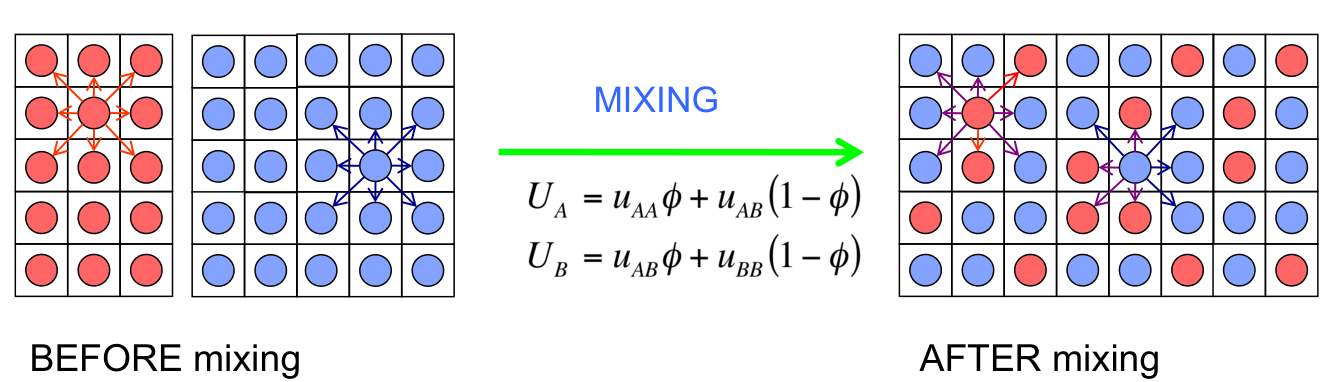
\includegraphics[width=90mm]{partA/Pictures/EnergyofMixing.png}
            \caption{Representation of the situation - before and after mixing}
            \label{fig: energy of mixing}
        \end{figure}
        where $\phi$ is the volume fraction of the substance $B$, and $(1-\phi)$ corresponds to the volume fraction of the substance $A$.\\

        Before mixing the molecules (ie, when the molecules are kept separated), the internal energy is given by
        \begin{equation}
            U_0 = \frac{zn}{2}\left[u_{AA}\phi+u_{BB}\left(1-\phi\right)\right]
        \end{equation}
        wheras after the process of mixing them, the total internal energy is
        \begin{equation}
            U = \frac{zn}{2}\left[U_A\phi+U_B\left(1-\phi\right)\right]
        \end{equation}
        such that
        \begin{equation}
            \Delta\overline{U}_{mix} = \frac{U-U_0}{n} = \frac{z}{2}\phi\left(1-\phi\right)\left(2u_{AB}-u_{AA}-u_{BB}\right)
        \end{equation}
        One defines the \color{purple}\textbf{Flory interaction parameter }\color{black} such that
        \begin{equation}
            x = \frac{z}{n}\frac{2u_{AB}-u_{AA}-u_{BB}}{k_BT}.
        \end{equation}
        It expresses the change in units of $k_BT$ gained when a molecule of $A$ is taken from an environment of pure $A$ and put intp an environment of pure $B$. The change in energy can then be written as
        \begin{equation}
            \Delta U_{mix} = x\phi\left(1-\phi\right)k_BT
        \end{equation}
        One can then express the change in free energy as
        \begin{equation}\label{eq: free energy mixture}
            \Delta F_{mix} = -T\Delta S_{mix} + \Delta U_{mix} = k_BT\left[\phi\log\phi+(1-\phi)\log\left(1-\phi\right)+x\phi\left(1-\phi\right)\right]
        \end{equation}
        \end{itemize}
    \end{example}

    \subsubsection{Flory-Huggins equation}

    \begin{theorem}[Flory-Huggins equation]
        Assuming that a mixture of two types of molecules can be expressed as in the mean field theory, ie it can be assumed that each individual molecule can be
        \begin{itemize}
            \item Arranged on a lattice, with each lattice location having $z$ direct neighbors,
            \item Composed of a mixture expressed in volume fractions $\phi_1,(...),\phi_n$
        \end{itemize}
        then the free energy of the mixture is expressed as \eqref{eq: free energy mixture}.
    \end{theorem}
    \begin{proof}
        See the second part of example \ref{ex: mixing of two liquids}.
    \end{proof}

    \begin{property}
        For all negative Flory-Huggins interaction parameters, the mean free energy of the mixture is negative for all $\phi$. In this case, mixing is favorable for all compositions.
    \end{property}
    \begin{property}
        When the Flory-Huggins parameter is positive, the equilibrium does not depends on the sign of $\Delta F_{mix}$ - rather, it depends on the $\Delta F_{mix}(\phi)$.
    \end{property}

    \begin{remark}
        In a real system, $x \approx A+\frac{B}{T}$.
    \end{remark}

    \paragraph{Concave curve scenario}

    \color{red} To be completed\color{black}

    \paragraph{Convex curve scenario}

    \color{red} To be completed\color{black}

    \paragraph{Stability of compositions}

    \color{red} To be completed\color{black}

    \paragraph{From free energy to phase diagrams}

    \color{red} To be completed\color{black}

    \part{Phase transitions II : Spinodal decomposition and solidification}

    \begin{abstract}
        In this part the mechanisms of equilibration of unstable and metastable systems is explained. For metastable systems, we study the process of nucleation and growth. For unstable systems, we study the spinodal decomposition.
    \end{abstract}

    \section{Mechanisms of phase transition}

    \begin{definition}[Spinodal decomposition]
        Continuous phase separation taking place in all the regions of a thermodynamic unstable sample. There is no thermodynamic barrier associated, thus we can treat it as a purely diffusive problem.    
    \end{definition}
    An example of such a situation is the demixing of liquids quenched together below/above the critical temperature (conversion of \textbf{unstable} phases).

    \begin{definition}[Homogeneous nucleation]
        Transformation occuring via the formation of nuclei and the growth of domains. Nuclei are created after overcoming a thermodynamic barrier, related to the balance of surface and volume energies. 
    \end{definition}
    An example of such a situation is the solidification from concentrated solutions (conversion of metastable phases, binodal decomposition).

    \begin{definition}
        Nucleation is here assisted by the presence of catalysers, increasing the rate of formation of new species (but not the growth!). Typical catalysers are surfaces of contaminants, powder or preformed crystals of the same material.  
    \end{definition}

    \subsection{Liquid-liquid transition - Spinodal decomposition}
    The tension surface $\gamma$ is defined as the ratio between the work necessary to build up a new surface, and the area of the surface itself.\\

    The free energy necessary to build up a spherical surcace of radius $R$ is 
    \begin{equation}
        \Delta G_{surf} = \gamma 4\pi R^2
    \end{equation}
    If the radius were to increase by $dR$, the free energy would increase by a factor
    \begin{equation}
        d\Delta G_{surf} = \gamma 8\pi RdR
    \end{equation}

    One deduces the expression of the Young-Laplace equation from this:
    \begin{align}
        \Delta p4\pi R^2dR = \gamma 8\pi RdR \quad \Rightarrow \quad \Delta p &= \gamma\left(\frac{1}{R_1}+\frac{1}{R_2}\right)
    \end{align}

    \color{red}\textbf{Discussion on wavelengths}\color{black}

    \subsubsection{Quantitative (phenomenological) picture}

    Phenomenologically, one has that the total free energy density must depend on:
    \begin{itemize}
        \item Local free energy;
        \item Gradient of composition (a term containing the square of concentration gradient).
    \end{itemize}

    Therefore, if $F$ denotes the density of free energy then
    \begin{equation}
        F \propto \int \left[f_0(\phi)+\kappa\left(\frac{d\phi}{dx}\right)^2\right]dx
    \end{equation}
    where $f_0$ is the free energy per unit volume for a uniform mixture, and $\kappa$ is the gradient energy coefficient, assumed constant in time.

    \paragraph{Fick's laws and spinodal}
    In the following paragraph, $J$ is the flux and $n$ is the density number.

    \begin{property}[Diffusion equation - Fick's $1^{st}$ law]
        \begin{equation}
            \bm{J} = -D\bm{\nabla}n
        \end{equation}
        where $D$ is \color{red}what is it?\color{black} a function of time with the final condition $D(t_f) = 0$.
    \end{property}
    
    \begin{property}[Continuity equation]
        \begin{equation}
            \frac{dn}{dt}+\bm{\nabla}\cdot\bm{J} = 0
        \end{equation}
    \end{property}

    \begin{property}[Fick's $2^{nd}$ law]
        \begin{equation}
            \frac{dn}{dt} = D\bm{\nabla}^2n
        \end{equation}
    \end{property}
    In this course, we will consider volume fraction and limit ourselves to the 1D-case. Hence, the properties can be rewritten as
    \begin{align}
        J &= -D\frac{d\phi}{dx}\\
        \frac{d\phi}{dt} &= -\frac{dJ}{dx}\label{eq: useful}\\
        \frac{d\phi}{dt} &= D\frac{d^2\phi}{dx^2}
    \end{align}

    \begin{property}[Modified diffusion equation]
        Let $J_A$ be the flux of species $A$, $M$ a positive transport coefficient (Onsager coefficient) and $\mu_A - \mu_B$ the exchange of chemical potential. It corresponds to the exchange of free energy by replacing an $A$-molecule by a $B$ molecule. Then,
        \begin{equation}
            J_A = -M\frac{d}{dx}\left(\mu_A-\mu_B\right)\label{eq: modified diffusion}
        \end{equation}
    \end{property}

    One can express $\mu$ by taking a derivative of the free-energy density:
    \begin{equation}
        \mu = \frac{d}{d\phi}\int \left[f_0(\phi)+\kappa\left(\frac{d\phi}{dx}\right)^2\right]dx
    \end{equation}
    The integral over this expression yields to 
    \begin{equation}
        \mu = \frac{df_0}{d\phi} + 2\kappa\frac{d^2\phi}{dx^2}
    \end{equation}
    Substituting in \eqref{eq: modified diffusion} results in
    \begin{equation}
        -J_A = \left(M\frac{d^2f_0}{d\phi^2}\right)\frac{d\phi}{dx} + \left(2M\kappa\right)\frac{d^3\phi}{dx^3}
    \end{equation}
    Combining this result and \eqref{eq: useful} yields to
    \begin{equation}
        \frac{\partial\phi(x,t)}{\partial t} = \underbrace{\left(Mf_0''\right)\frac{\partial^2\phi}{\partial x^2}}_{\text{Diffusion equation}}+\overbrace{\left(2M\kappa\right)\frac{\partial^4\phi}{\partial x^4}}^{\text{Gradient term}}
    \end{equation}
    This is the \color{purple}\textbf{Cahn-Hillard equation}\color{black}. It is often written as
    \begin{equation}
        \frac{\partial\phi(x,t)}{\partial t} = D_{eff}\frac{\partial^2\phi}{\partial x^2}+\left(2M\kappa\right)\frac{\partial^4\phi}{\partial x^4}
    \end{equation}
    The solution to this equation can be written as 
    \begin{equation}
        \phi(x,t) = \phi_0 + A\cos\left(qx\right)\exp\left[\underbrace{-D_{eff}q^2\left(1+\frac{2\kappa q^2}{f''_0}\right)t}_{\text{Amplification factor } R(q)}\right]
    \end{equation}

    \color{red}\textbf{Discussion on the solution }\color{black}

    \subsection{Liquid-solid transition - Homogeneous nucleation}
    The liquid-liquid transition could be described in terms of the change of one parameter (density) : this is not possible in the liquid-solid equivalent, as it would require the consideration of an infinite number of order parameters. Thus, the treatement is mostly phenomenological.\\

    In the process of solidification, there is a reduction of free energy (gain) but also a non-negligeable loss in the formation of the interfaces. How can we form crystals at $T_m$ ? Using the same approach as for the binodal decomposition and assuming the spontaneous appearance of a spherical crystal nucleus of radius $r$,
    \begin{align}
        \Delta G(r) &= \frac{4}{3}\pi r^3\Delta G_{\color{red}r\color{black}}+4\pi r^2\gamma_{sl}\\
        \Delta S_m &= \left(\frac{\partial G_s}{\partial T}\right)_{P} - \left(\frac{\partial G_l}{\partial T}\right)_P = \frac{\Delta H_m}{T_m}
    \end{align}
    To initiate the process of crystalization, one has to undercool the melt by a small value $\Delta T$ - the free energy change upon freezing becomes (assuming constant derivative)
    \begin{equation}
        \Delta G_b = -\frac{\Delta H_m}{T_m}\Delta T
    \end{equation}
    \paragraph{Analysis of the solution}
    The free energy change when the crystal nucleus of radius $r$ appears is then
    \begin{equation}
        \Delta G(r) = -\frac{4}{3}\pi r^3\frac{\Delta H_m}{T_m}\Delta T+4\pi r^2\gamma_{sl}
    \end{equation}
    One shows that the maximum of $\Delta G(r)$ is at $r^* = \frac{2\gamma_{sl}T_m}{\Delta H_m\Delta T}$. The maximum is then
    \begin{equation}
        \Delta G^* = \frac{16\pi}{3}\gamma_{sl}^3\left(\frac{T_m}{\Delta H_m}\right)^2\frac{1}{\Delta T^2}
    \end{equation}
    If the nuclei is bigger than $r^*$, it will continue to grow: it is said to be a stable nuclei. Conversly, if it is smaller than $r^*$ is will shrink until it is gone. It is said to be an unstable nuclei.

    \subsection{Liquid-solid transition - Heteregeneous nucleation}

    \color{red}\textbf{To be completed}\color{black}


\end{document}